\documentclass[11pt]{article}

%------------------------- fonts & encoding -----------------------------------
\usepackage[T1]{fontenc}
\usepackage[utf8]{inputenc}
\usepackage{amsmath,amssymb,amsthm}
\usepackage{mathtools}
\usepackage[sc]{mathpazo}
\linespread{1.06}
\usepackage{microtype}

%------------------------- layout ---------------------------------------------
\usepackage[a4paper,margin=1.05in,marginparwidth=1.0in]{geometry}
\usepackage{booktabs}
\usepackage{enumitem}
\setlist{itemsep=2pt,topsep=3pt}
\usepackage{xcolor}
\usepackage{graphicx}
\usepackage{tikz}
\usepackage{pgfplots}
\pgfplotsset{compat=1.17}
\usepackage[most,breakable]{tcolorbox}

%------------------------- palette --------------------------------------------
\definecolor{crimson}{HTML}{A51C30}
\definecolor{ink}{HTML}{1A1A1A}
\definecolor{steel}{HTML}{2C5F8A}
\definecolor{amber}{HTML}{9A6A00}
\definecolor{teal}{HTML}{1F6F6B}
\definecolor{paperlt}{HTML}{F7F4EF}

%------------------------- section styling ------------------------------------
\usepackage{titlesec}
\titleformat{\section}{\Large\bfseries\color{steel}}{\thesection}{0.7em}{}
\titleformat{\subsection}{\large\bfseries\color{ink}}{\thesubsection}{0.6em}{}
\titlespacing*{\section}{0pt}{1.6em}{0.6em}

%------------------------- hyperref -------------------------------------------
\usepackage[colorlinks=true,linkcolor=steel,citecolor=steel,urlcolor=crimson]{hyperref}

%------------------------- theorem environments -------------------------------
\theoremstyle{definition}
\newtheorem{definition}{Definition}[section]
\newtheorem{example}{Example}[section]
\newtheorem{exercise}{Exercise}[section]
\theoremstyle{plain}
\newtheorem{proposition}{Proposition}[section]
\theoremstyle{remark}
\newtheorem*{remark}{Remark}

%------------------------- callout boxes --------------------------------------
\newtcolorbox{intuition}{
  enhanced, breakable, colback=crimson!5, colframe=crimson, boxrule=0.5pt,
  left=8pt,right=8pt,top=6pt,bottom=6pt, arc=2pt,
  colbacktitle=crimson, coltitle=paperlt, fonttitle=\bfseries, title={Intuition}}

\newtcolorbox{pitfall}{
  enhanced, breakable, colback=amber!7, colframe=amber, boxrule=0.5pt,
  left=8pt,right=8pt,top=6pt,bottom=6pt, arc=2pt,
  colbacktitle=amber, coltitle=paperlt, fonttitle=\bfseries, title={Pitfall}}

\newtcolorbox{keyresult}{
  enhanced, breakable, colback=steel!6, colframe=steel, boxrule=0.5pt,
  left=8pt,right=8pt,top=6pt,bottom=6pt, arc=2pt,
  colbacktitle=steel, coltitle=paperlt, fonttitle=\bfseries, title={Takeaway}}

\newtcolorbox{observed}{
  enhanced, breakable, colback=teal!6, colframe=teal, boxrule=0.5pt,
  left=8pt,right=8pt,top=6pt,bottom=6pt, arc=2pt,
  colbacktitle=teal, coltitle=paperlt, fonttitle=\bfseries, title={Measured}}

%------------------------- math operators -------------------------------------
\DeclareMathOperator{\Var}{Var}
\DeclareMathOperator{\Cov}{Cov}
\DeclareMathOperator{\Corr}{corr}
\DeclareMathOperator{\diag}{diag}
\DeclareMathOperator{\std}{std}
\DeclareMathOperator*{\avg}{\mathbb{E}}
\newcommand{\T}{^{\!\top}}
\newcommand{\R}{\mathbb{R}}
\newcommand{\half}{\tfrac12}
\newcommand{\wvec}{\mathbf{w}}
\newcommand{\Xmat}{\mathbf{X}}
\newcommand{\Fmat}{\mathbf{F}}
\newcommand{\Vmat}{\mathbf{V}}
\newcommand{\Umat}{\mathbf{U}}
\newcommand{\Rmat}{\mathbf{R}}
\newcommand{\Lam}{\boldsymbol{\Lambda}}
\newcommand{\Del}{\boldsymbol{\Delta}}
\newcommand{\fvec}{\mathbf{f}}

%------------------------- title ----------------------------------------------
\title{\vspace{-2.2em}
  {\color{steel}\rule{\textwidth}{1.3pt}}\\[0.7em]
  \Huge\bfseries The USE4 Risk Model, End to End\\[0.35em]
  \large\mdseries The assembly line from data to a portfolio risk forecast\\[0.4em]
  {\color{steel}\rule{\textwidth}{0.7pt}}}
\author{}
\date{}

%------------------------- watermark footer -----------------------------------
\usepackage{fancyhdr}
\pagestyle{fancy}
\fancyhf{}
\renewcommand{\headrulewidth}{0pt}
\renewcommand{\footrulewidth}{0pt}
\fancyfoot[L]{\footnotesize\color{black!45}MSCI Barra USE4 Imitation}
\fancyfoot[R]{\footnotesize\color{black!45}\thepage}

\begin{document}
\maketitle
\thispagestyle{empty}

\begin{abstract}
A risk model answers one practical question: how much will this portfolio's value bounce around, and where does that uncertainty come from? Forecasting the full covariance of thousands of stocks directly is hopeless---the matrix has millions of entries and far too little data to estimate them. The USE4 model sidesteps this by asserting that nearly all co-movement is driven by a few dozen shared factors: a market/country factor, industry membership, and a handful of measurable style tilts. Each stock's return is its exposure to those factors times the factors' returns, plus an idiosyncratic remainder, and the asset covariance collapses to $V = \Xmat\Fmat\Xmat\T + \Del$, a low-rank factor piece plus a diagonal of stock-specific variances. From this, any portfolio's variance splits cleanly into factor risk and specific risk, $\sigma_p^2 = \wvec\T\Xmat\Fmat\Xmat\T\wvec + \wvec\T\Del\wvec$, which is the governing identity of everything that follows. This note maps the assembly line that builds the four objects $\Xmat$, $\fvec$ (with its residual $u$), $\Fmat$, and $\Del$, and composes them into that one number. The emphasis is conceptual: why each stage exists, what it produces, and how the stages chain so that the cap-weighted market turns out to be almost pure country risk while a momentum tilt turns out to be almost pure style risk.
\end{abstract}

\begin{tcolorbox}[colback=paperlt,colframe=ink!30,boxrule=0.4pt,arc=2pt,left=10pt,right=10pt,top=8pt,bottom=8pt]
\textbf{How to read these notes.} Read this document top to bottom as a tour of one pipeline. Section~\ref{sec:goal} states the single identity that the whole model serves; Sections~\ref{sec:data}--\ref{sec:specific} walk the assembly line left to right (data, exposures $\Xmat$, the regression that yields factor returns $\fvec$ and specific returns $u$, the factor covariance $\Fmat$, and the specific diagonal $\Del$); Section~\ref{sec:decomp} composes them back into portfolio risk and attribution; Section~\ref{sec:caveat} recaps the line and gives a caveat. The numbers labelled as measured come from a single run of our personal build. Four coloured boxes recur: \textcolor{crimson}{\textbf{Intuition}} gives the mental picture, \textcolor{amber}{\textbf{Pitfall}} flags what breaks without the fix, \textcolor{steel}{\textbf{Takeaway}} states a load-bearing result, and \textcolor{teal}{\textbf{Measured}} reports real numbers from the build run.

\smallskip
\textbf{Reference material.}
\begin{itemize}[leftmargin=1.4em,topsep=2pt]
  \item External: Menchero, Orr \& Wang (2011), USE4 Methodology Notes \& Empirical Notes; Menchero, Wang \& Orr (2011), eigen-adjusted covariance.
\end{itemize}
\end{tcolorbox}

\tableofcontents
\bigskip

\section{What the risk model is, and the one identity}\label{sec:goal}

\paragraph{Learning objectives.}
\begin{itemize}[leftmargin=1.4em,nosep]
  \item Write the return decomposition $r = \Xmat\fvec + u$ and the asset covariance $V = \Xmat\Fmat\Xmat\T + \Del$ from memory, and say which assumptions make the second follow from the first.
  \item Split a portfolio's variance into a factor part and a specific part.
  \item Name the four built objects and say which stage produces each.
\end{itemize}

The model exists to forecast the covariance of returns for \emph{any} portfolio of US equities. If we had a reliable $N\times N$ covariance matrix for $N\approx 2{,}500$ stocks, every portfolio variance would follow from $\sigma_p^2 = \wvec\T V \wvec$. But a raw sample covariance over thousands of names is rank-deficient and wildly noisy---there are roughly three million distinct entries and only a few hundred monthly observations. The structural move is to insist that returns share a small number of common drivers.

\begin{definition}[Factor decomposition of returns]
For each stock $i$ in each period, the excess return decomposes as
\[
  r_i = \sum_{k=1}^{K} X_{ik}\, f_k + u_i,
\]
where $X_{ik}$ is stock $i$'s \emph{exposure} to factor $k$, $f_k$ is the \emph{factor return} (common to all stocks), and $u_i$ is the \emph{specific} (idiosyncratic) return. In matrix form, $r = \Xmat\fvec + u$.
\end{definition}

Assume the specific returns are mutually uncorrelated and uncorrelated with the factors. Then the asset covariance inherits the same low-rank-plus-diagonal structure:
\[
  V \;=\; \Xmat\,\Fmat\,\Xmat\T \;+\; \Del,
\]
where $\Fmat = \Cov(\fvec)$ is the $K\times K$ factor-return covariance and $\Del = \diag(\Var(u_i))$ is the diagonal of specific variances. Here $K\approx 68$, so $\Xmat\Fmat\Xmat\T$ has rank at most $68$ no matter how many stocks there are; the heavy lifting moves from an unmanageable $N\times N$ object to a small, well-conditioned $\Fmat$ plus $N$ separate scalars.

\begin{example}[The identity on two stocks and one factor]
Take $N=2$, $K=1$, exposures $\Xmat=\begin{psmallmatrix}1\\2\end{psmallmatrix}$, factor variance $\Fmat=[\,0.04\,]$, and specific variances $\Del=\diag(0.01,\,0.09)$. Then
\[
  V=\Xmat\Fmat\Xmat\T+\Del=\begin{psmallmatrix}0.04 & 0.08\\ 0.08 & 0.16\end{psmallmatrix}+\begin{psmallmatrix}0.01 & 0\\ 0 & 0.09\end{psmallmatrix}=\begin{psmallmatrix}0.05 & 0.08\\ 0.08 & 0.25\end{psmallmatrix}.
\]
The off-diagonal covariance $0.08$ is purely the shared factor ($X_1 X_2 F$); the diagonal adds each stock's own variance. An equal-weight portfolio $\wvec=(\half,\half)$ has $\sigma_p^2=\wvec\T V\wvec = 0.1125$, of which $\wvec\T\Xmat\Fmat\Xmat\T\wvec=0.09$ is factor risk and $\wvec\T\Del\wvec=0.025$ is specific. The whole model is this picture at scale.
\end{example}

Multiplying through by portfolio weights gives the identity that the entire pipeline serves.

\begin{keyresult}
\[
  \boxed{\;\sigma_p^2 \;=\; \underbrace{\wvec\T \Xmat \Fmat \Xmat\T \wvec}_{\text{factor risk}} \;+\; \underbrace{\wvec\T \Del\, \wvec}_{\text{specific risk}}\;}
\]
Every portfolio's variance is a factor part plus a specific part. The four objects $\Xmat$, $\Fmat$, $\Del$ (and the regression that ties $\fvec$ and $u$ to $\Xmat$) are what the assembly line builds.
\end{keyresult}

\begin{intuition}
A few dozen shared drivers---being a US stock at all, belonging to an industry, leaning value or momentum---explain most of why stocks move together. What is left after subtracting those is each company's own news, which is roughly independent across names and therefore \emph{diversifies away} in a broad portfolio. So the factor part dominates concentrated tilts, while the specific part shrinks toward zero as you hold more names. The model is an assembly line: data feeds exposures, exposures feed a regression, the regression's outputs feed two covariance estimators, and those compose back into one risk number.
\end{intuition}

\begin{exercise}
Derive $V = \Xmat\Fmat\Xmat\T + \Del$ by expanding $\Cov(\Xmat\fvec+u,\,\Xmat\fvec+u)$. State exactly where you use $\Cov(\fvec,u)=0$ and where you use $\Cov(u_i,u_j)=0$ for $i\neq j$. (Hint: covariance is bilinear; the two cross terms vanish, and the specific term keeps only its diagonal.)
\end{exercise}

\begin{exercise}
Suppose a portfolio is built factor-neutral, $\wvec\T\Xmat = 0$. Show its variance reduces to $\wvec\T\Del\wvec$, and that for an equal-weight book of $n$ names with bounded specific variances this falls like $1/n$. (Hint: the factor quadratic form is exactly zero; average $n$ independent variances scaled by $1/n^2$.)
\end{exercise}

The remainder of the note walks that line. We first secure the data and the universe, then build $\Xmat$, then run the regression that produces $\fvec$ and $u$, then estimate $\Fmat$ and $\Del$, and finally compose $\sigma_p$ and attribute it. Figure~\ref{fig:pipeline} is the map.

\begin{figure}[htbp]
\centering
\resizebox{\linewidth}{!}{%
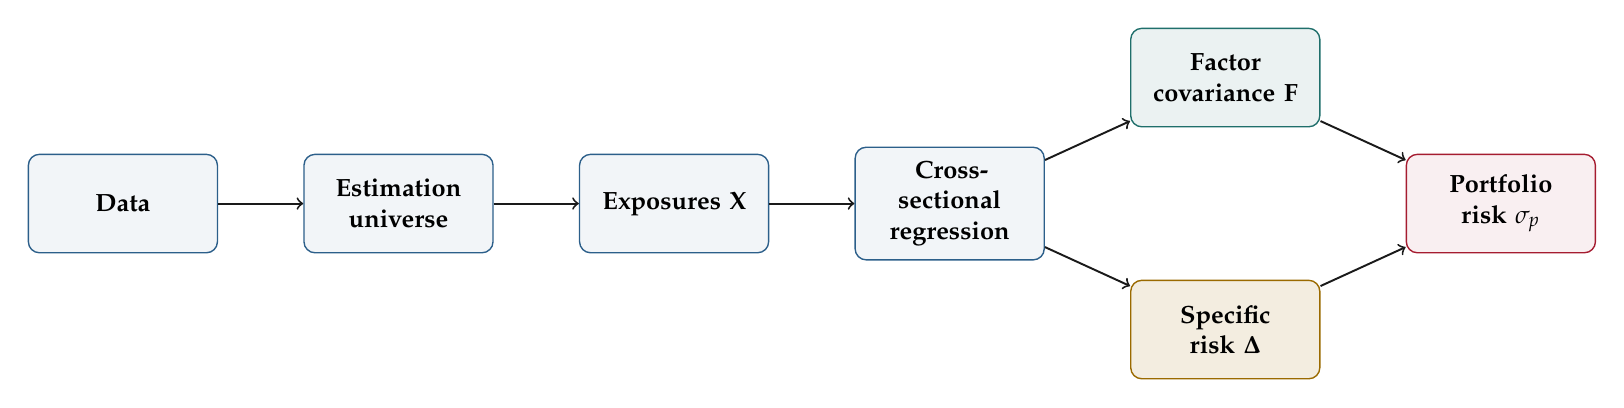
\begin{tikzpicture}[font=\small,
  box/.style={draw, rounded corners, align=center, text width=2.05cm, inner sep=5pt,
              minimum height=1.25cm, fill=steel!6, draw=steel, line width=0.5pt}]
  \node[box] (data) at (0,0)    {\textbf{Data}};
  \node[box] (estu) at (3.5,0)  {\textbf{Estimation universe}};
  \node[box] (expo) at (7.0,0)  {\textbf{Exposures} $\Xmat$};
  \node[box] (csr)  at (10.5,0) {\textbf{Cross-sectional regression}};
  \node[box, fill=teal!9, draw=teal]       (fcov) at (14.0,1.6)  {\textbf{Factor covariance} $\Fmat$};
  \node[box, fill=amber!12, draw=amber]    (spec) at (14.0,-1.6) {\textbf{Specific risk} $\Del$};
  \node[box, fill=crimson!7, draw=crimson] (risk) at (17.5,0)    {\textbf{Portfolio risk} $\sigma_p$};
  \draw[->,line width=0.7pt,draw=ink] (data)--(estu);
  \draw[->,line width=0.7pt,draw=ink] (estu)--(expo);
  \draw[->,line width=0.7pt,draw=ink] (expo)--(csr);
  \draw[->,line width=0.7pt,draw=ink] (csr)--(fcov);
  \draw[->,line width=0.7pt,draw=ink] (csr)--(spec);
  \draw[->,line width=0.7pt,draw=ink] (fcov)--(risk);
  \draw[->,line width=0.7pt,draw=ink] (spec)--(risk);
\end{tikzpicture}}
\caption{The assembly line. Data and the estimation universe feed the exposure matrix $\Xmat$; a $\sqrt{\text{mcap}}$-weighted cross-sectional regression each period yields factor returns $\fvec$ and specific returns $u$; these feed the factor covariance $\Fmat$ and the specific diagonal $\Del$, which compose into portfolio risk $\sigma_p^2 = \wvec\T\Xmat\Fmat\Xmat\T\wvec + \wvec\T\Del\wvec$.}
\label{fig:pipeline}
\end{figure}

\begin{remark}
The whole gain is that $K=68 \ll N\approx 2{,}500$. A direct $N\times N$ sample covariance has far more free entries than data points and is wildly unstable; a $68\times 68$ factor covariance is comfortably over-determined by the same return history, which is why $\Fmat$ can be estimated honestly while $V$ cannot.
\end{remark}

\section*{Notation}
\addcontentsline{toc}{section}{Notation}

\begin{center}
\small
\begin{tabular}{@{}ll@{}}
\toprule
Symbol & Meaning \\
\midrule
$r,\ r_i$ & excess (log) return; for stock $i$ \\
$\Xmat,\ X_{ik}$ & exposure matrix ($N\times K$); exposure of stock $i$ to factor $k$ \\
$\fvec,\ f_k$ & factor-return vector; return of factor $k$ \\
$u,\ u_i$ & specific (idiosyncratic) return vector; for stock $i$ \\
$\Fmat$ & factor-return covariance ($K\times K$) \\
$\Del$ & specific-variance diagonal ($N\times N$) \\
$\Vmat,\ V$ & asset covariance $=\Xmat\Fmat\Xmat\T+\Del$ \\
$\wvec$ & portfolio weight vector; ``the market'' is the ESTU cap-weighted $\wvec$ \\
$\sigma_p$ & portfolio volatility \\
$N$ & number of assets ($\approx 2{,}500$) \\
$K$ & number of factors ($=68$: country $+$ 55 industries $+$ 12 styles) \\
$m_{i,t}$ & total market capitalisation of stock $i$ at date $t$ \\
$W$ & WLS weight matrix, $\diag(\sqrt{m_{i,t}})$ \\
$R^2$ & per-period cross-sectional coefficient of determination \\
$\Var,\Cov,\Corr$ & variance, covariance, correlation \\
$\diag(\cdot),\ \std,\ \avg$ & diagonal-extraction; standard deviation; average \\
$(\cdot)\T$ & transpose \\
\bottomrule
\end{tabular}
\end{center}

\section{Data foundation and point-in-time discipline}\label{sec:data}

\paragraph{Learning objectives.}
\begin{itemize}[leftmargin=1.4em,nosep]
  \item Name the raw inputs and the single shared return artifact they feed.
  \item Explain what ``point-in-time'' means operationally.
  \item Say why look-ahead inflates in-sample fit yet vanishes in live use.
\end{itemize}

Every downstream number rests on prices, fundamentals, and a risk-free rate. The build draws prices and corporate fundamentals from Sharadar (the SEP price file and the SF1 fundamentals file) and the risk-free rate from Ken French's data library. From these it constructs one shared artifact---a daily \emph{excess log-return} panel---that every later stage consumes, so that the universe, the descriptors, the regression, and both covariance estimators all speak the same return language.

The non-negotiable discipline is \emph{point-in-time} (PIT) construction: at any historical date the model may use only information that was actually knowable then. Fundamentals are stamped by their filing date (the \texttt{datekey}), not the period they describe, and are allowed to persist only inside a staleness window of about a year and a half before a stock is treated as missing that descriptor. Benchmark weights---the ESTU cap weights introduced in the next section---enter lagged.

\begin{pitfall}
A single peeked value---using a fiscal-year figure on a date before it was filed, or this month's index weights to explain this month's returns---creates correlation that exists only because you cheated. A leaked filing date can add several points of phantom in-sample $R^2$. In-sample fit then looks excellent and the model collapses in live trading, where the future genuinely is not available: you have built a model that partly memorised the future. PIT discipline is what makes the back-test an honest estimate of forward performance rather than a flattering illusion.
\end{pitfall}

\begin{exercise}
A descriptor uses trailing-twelve-month earnings. Explain why aligning it to the fiscal period end rather than the filing date leaks information, and estimate the typical leak in calendar days. (Hint: think about the gap between period end and the 10-K/10-Q filing.)
\end{exercise}

\section{Exposures: the estimation universe and the factor cross-section}\label{sec:expo}

\paragraph{Learning objectives.}
\begin{itemize}[leftmargin=1.4em,nosep]
  \item State what the estimation universe is and three things it fixes.
  \item List the three blocks of $\Xmat$ and their column counts.
  \item Explain the standardisation convention and why it makes the cap-weighted market style-neutral.
\end{itemize}

\paragraph{The estimation universe.} Before any factor can be measured, the model fixes a coherent set of stocks---the \emph{estimation universe} (ESTU), a first-principles proxy for the MSCI USA IMI, targeting about 99\% of US float market capitalisation, roughly $2{,}500$ names. The ESTU is load-bearing far beyond ``which stocks to include'': it is the sample over which descriptors are standardised (so it fixes the standardisation moments), it is the benchmark whose cap weights define ``the market,'' and it is the regression sample each period. Its construction uses a low-hundreds-of-millions-of-dollars size floor, a fixed top-$N$ target (a few thousand names), an asymmetric rank buffer to damp turnover, and a minimum-populated-window rule for adequate history.

\paragraph{The exposure matrix.} With the universe fixed, $\Xmat$ is assembled from three blocks, $68$ columns in all:
\begin{itemize}[leftmargin=1.4em,nosep]
  \item \textbf{Country} (1 column): a constant equal to one for every stock---the market/country factor every US equity loads on.
  \item \textbf{Industries} (55 columns): hand-engineered industry membership, essentially one-hot, so each stock carries its sector's common return.
  \item \textbf{Styles} (12 columns): measurable tilts---size, book-to-price, momentum, residual volatility, leverage, liquidity, earnings yield, dividend yield, growth, non-linear size, non-linear beta, and beta.
\end{itemize}

The twelve styles share one skeleton: form a raw descriptor, trim its extreme tails, orthogonalise it where it would otherwise duplicate another factor, and standardise. Standardisation is to \emph{cap-weighted mean zero and equal-weighted unit standard deviation} over the ESTU. The canonical shipped model is \emph{estimate-free}: where a descriptor cannot be computed for a stock, the exposure is simply absent and the standardisation and coverage rules handle it, rather than imputing the value from a model.

\begin{intuition}
Cap-weighting the mean to zero means the market portfolio has zero exposure to every style by construction. So when the regression runs, the market's return is absorbed entirely by the country factor, and styles describe only \emph{deviations} from the market---a value tilt, a small-cap tilt. That is exactly the behaviour we want: the cap-weighted market is style-neutral, and style factors carry the cross-sectional spread.
\end{intuition}

\begin{exercise}
Show that if a style descriptor has cap-weighted mean zero over the ESTU, then the ESTU cap-weighted portfolio (``the market'') has zero exposure to that style. (Hint: the portfolio's exposure is the cap-weighted average of the column.)
\end{exercise}

\section{Factor and specific returns: the cross-sectional regression}\label{sec:csr}

\paragraph{Learning objectives.}
\begin{itemize}[leftmargin=1.4em,nosep]
  \item Describe the weighted cross-sectional regression and its weights.
  \item Explain the industry constraint and why it is needed.
  \item Recall the empirical shape of factor-return volatilities and correlations.
\end{itemize}

Exposures are observed; factor returns are not. Each period the model recovers them with a \emph{single} cross-sectional regression. Stack that period's stock excess returns in $r$, regress on $\Xmat$ by weighted least squares with weights proportional to $\sqrt{m_{i,t}}$, and read off the fitted coefficients as the factor returns $\fvec$; the residuals are the specific returns $u$:
\[
  \hat{\fvec} = (\Xmat\T W \Xmat)^{-1}\Xmat\T W\, r, \qquad u = r - \Xmat\hat{\fvec}, \qquad W = \diag(\sqrt{m_{i,t}}).
\]
That is, the fit minimises the cap-rooted weighted sum of squared specific returns, $\sum_i \sqrt{m_{i,t}}\, u_i^2$. Square-root-cap weighting is a compromise: it lets larger, better-measured stocks anchor the fit without letting a handful of mega-caps dominate, and it stabilises the residual variance across the size spectrum.

\begin{intuition}
A time-series regression runs \emph{down} a single stock's history to estimate its loadings. This regression runs \emph{sideways}: at one instant, across all stocks at once, it asks what single set of factor returns best explains today's cross-section of moves given each stock's known exposures. Run the regression sideways, period by period, and you recover a time series of factor returns without ever assuming a stock's loadings are constant.
\end{intuition}

\paragraph{Identification.} The country column is a vector of ones, and the $55$ industry columns sum, stock by stock, to that same vector of ones---so country and industries are exactly collinear unless we break the tie. USE4 imposes a constraint: the cap-weighted sum of industry factor returns is zero. Country then carries the market-wide move and each industry carries its return \emph{relative} to the market, with country$+$industries no longer rank-deficient.

\begin{observed}
On the personal build (factor-return panel through 2026-04-30), the cross-section runs over roughly $303$ monthly transitions with mean cross-sectional $R^2 \approx 0.25$ and a maximum design condition number near $50$. The recovered country factor return correlates with the cap-weighted market at $0.998$ (USE4 reports about $0.999$), and the industry constraint holds to about $1\mathrm{e}{-18}$---numerically exact.
\end{observed}

The \emph{structure} of the recovered factor returns matches USE4: country dominates, beta couples tightly to the market, and the styles are small and nearly orthogonal to one another. Figures~\ref{fig:volhier} and~\ref{fig:corr} show the volatility hierarchy and the correlation structure.

\begin{figure}[htbp]
\centering

\includegraphics[width=\linewidth]{figures/csr_vol_hierarchy.png}
\caption{Annualized factor-return volatilities (personal build, factor-return panel through 2026-04-30). The country factor ($\approx 16\%$) dwarfs the styles; beta ($\approx 8\%$) and momentum ($\approx 4\%$) lead the rest, which sit near $2$--$3\%$. The amber band is the 55-industry range (median $\approx 12\%$).}
\label{fig:volhier}
\end{figure}

\begin{observed}
Annualised factor-return volatilities (personal build): country $16.1\%$ towers over everything; beta $8.0\%$; then momentum $4.4\%$, residual volatility $3.6\%$, leverage $2.7\%$, size $2.6\%$, book-to-price $2.6\%$, earnings yield $2.4\%$, non-linear size $2.2\%$, dividend yield $2.1\%$, liquidity $2.0\%$, non-linear beta $1.9\%$, and growth $1.2\%$. The $55$ industries have median vol $12.0\%$ (range $6.5\%$--$28.0\%$). Cross-factor correlations are modest: $\Corr(\text{beta},\text{country})=0.78$, the largest style--style correlation is $0.47$, and the factor-correlation condition number is $19.4$.
\end{observed}

\begin{figure}[htbp]
\centering

\includegraphics[width=0.82\linewidth]{figures/csr_factor_corr.png}
\caption{Monthly factor-return correlations (country $+$ 12 styles, personal build). Beta couples to the country factor ($+0.78$) while the styles stay near-orthogonal (max off-diagonal $\approx 0.47$), so the design stays well-conditioned. This is the structure the factor covariance $\Fmat$ must capture.}
\label{fig:corr}
\end{figure}

\begin{exercise}
The mean cross-sectional $R^2$ is about $0.25$. Argue why a \emph{low} per-period $R^2$ is compatible with the factor model explaining most of the \emph{covariance}, even though it explains only a quarter of the cross-sectional return variance. (Hint: idiosyncratic shocks are large but uncorrelated, so they dominate cross-sectional variance yet contribute almost nothing to covariance.)
\end{exercise}

\begin{exercise}
$\Corr(\text{beta},\text{country})=0.78$ is high, yet beta is kept as a separate factor rather than folded into country. Explain why country, being a column of ones, has zero cross-sectional dispersion and so cannot capture the spread in market sensitivity that beta measures. (Hint: a constant column distinguishes no two stocks.)
\end{exercise}

\section{The factor covariance \texorpdfstring{$\Fmat$}{F}}\label{sec:fcov}

\paragraph{Learning objectives.}
\begin{itemize}[leftmargin=1.4em,nosep]
  \item Name the four corrections layered into $\Fmat$ and what each fixes.
  \item Explain why an optimiser punishes an under-forecast covariance.
  \item State what eigenfactor de-biasing does to the bias statistic.
\end{itemize}

Having a time series of factor returns $\fvec$, the model forecasts their $K\times K$ covariance $\Fmat$. A raw sample covariance is biased and unstable, so four corrections are layered on:
\begin{enumerate}[leftmargin=1.6em,nosep]
  \item \textbf{EWMA volatility and correlation.} Exponentially weighted moving averages let recent observations matter more. Volatilities and correlations are estimated \emph{separately}---a shorter half-life for the volatilities and a longer one for the correlation matrix, then recombined into the covariance---because volatility moves faster than co-movement.
  \item \textbf{Newey--West autocorrelation correction.} Monthly factor returns carry serial correlation; ignoring it understates longer-horizon variance. The Newey--West adjustment folds in the lagged autocovariances.
  \item \textbf{Eigenfactor de-biasing} (Menchero, Wang \& Orr 2011). The sample's own eigen-portfolios have systematically biased variances---the most diversified directions are forecast too calm. Simulation calibrates a multiplier per eigen-direction that flattens this bias.
  \item \textbf{Volatility-regime scaler.} A final level adjustment so the overall forecast tracks the prevailing volatility regime rather than a long-run average.
\end{enumerate}

\begin{intuition}
Why obsess over the covariance being right rather than merely reasonable? Because a mean--variance optimiser actively \emph{seeks out} directions the model thinks are cheap. If $\Fmat$ under-forecasts the variance of some eigen-portfolio, the optimiser loads on it precisely because it looks like free risk reduction---a phantom safe direction---and the realised risk then overshoots. Every correction here is a defence against an optimiser exploiting the model's blind spots.
\end{intuition}

\begin{observed}
The build produces $68\times 68$ symmetric positive-semidefinite forecasts. Eigenfactor de-biasing cuts the mean absolute bias $|{\text{bias}}-1|$ across eigen-directions from $0.31$ to $0.07$ (personal build).
\end{observed}

Figure~\ref{fig:corr} also shows the correlation structure $\Fmat$ must reproduce: the strong beta--country link and the otherwise near-diagonal style block.

\begin{exercise}
A ``bias statistic'' is the realised volatility of an eigen-portfolio divided by its forecast, averaged over time; a well-calibrated forecast gives one. Explain why the most diversified (smallest-forecast-variance) eigen-portfolios tend to have a bias statistic \emph{above} one, and why that under-forecast is the dangerous direction for an optimiser. (Hint: sample estimation disperses eigenvalues, pushing the smallest forecast variances too low; an optimiser loads on whatever looks cheapest.)
\end{exercise}

\section{The specific risk diagonal \texorpdfstring{$\Del$}{Delta}}\label{sec:specific}

\paragraph{Learning objectives.}
\begin{itemize}[leftmargin=1.4em,nosep]
  \item Distinguish the time-series and structural specific-risk models and say when each applies.
  \item Explain why thin-history small caps need a structural fallback.
  \item Describe the empirical-Bayes shrinkage toward size peers.
\end{itemize}

The other built object is $\Del$, the diagonal of idiosyncratic variances, one per stock, estimated from the specific returns $u$ the regression left behind. Two estimators feed it:
\begin{itemize}[leftmargin=1.4em,nosep]
  \item A \textbf{time-series model}: an EWMA of squared specific returns with a Newey--West correction, for stocks with enough history to estimate their own idiosyncratic volatility directly.
  \item A \textbf{structural model}: a cross-sectional regression of log specific volatility on style exposures, which predicts a plausible specific vol for a stock from its characteristics alone---essential for names with too little history to trust their own sample.
\end{itemize}
The two are blended, and the result is empirical-Bayes \emph{shrunk} toward the average of size peers, pulling noisy individual estimates toward their cohort.

\begin{intuition}
Small caps are exactly the stocks with short, gappy return histories---so their own sample specific vol is the least trustworthy just when it matters. The structural model says ``a stock that looks like this usually has specific vol about that,'' and shrinkage borrows strength from similar-sized peers. The blend trusts a stock's own history when it is long and informative, and leans on its characteristics when it is not.
\end{intuition}

\begin{observed}
On the personal build the overall cap-weighted specific-risk bias is about $1.07$, and the bias spread across size deciles is only about $0.09$---essentially flat, meaning the model is not systematically wrong for small versus large stocks.
\end{observed}

\begin{exercise}
The mean squared error of an estimator decomposes as $\text{MSE}=\text{bias}^2+\text{variance}$. For a thin-history small cap, explain which of the two terms empirical-Bayes shrinkage toward size peers is designed to reduce, and why accepting a little of the other term is worth it. (Hint: a noisy own-sample estimate is nearly unbiased but high-variance; the peer mean trades a touch of bias for a large variance cut.)
\end{exercise}

\section{Putting it together: portfolio risk and attribution}\label{sec:decomp}

\paragraph{Learning objectives.}
\begin{itemize}[leftmargin=1.4em,nosep]
  \item Compose $\sigma_p$ from the four objects.
  \item State the per-asset Pythagorean identity.
  \item Explain Euler attribution and read a portfolio's risk composition.
\end{itemize}

All four objects now exist, and the identity composes them:
\[
  \sigma_p \;=\; \sqrt{\,\wvec\T \Xmat \Fmat \Xmat\T \wvec \;+\; \wvec\T \Del\, \wvec\,}.
\]
At the single-asset level the same split is Pythagorean: each stock's $\text{factor}^2 + \text{specific}^2 = \text{total}^2$, where the factor part for stock $i$ is the $i$-th diagonal entry of $\Xmat\Fmat\Xmat\T$. To distribute the portfolio's risk across factor groups, use \emph{Euler attribution}: because $\sigma_p$ is homogeneous of degree one in $\wvec$, it equals the sum of each position's marginal-times-holding contribution, and these contributions group exactly into country, industry, style, and specific buckets that sum to $\sigma_p$.

\begin{figure}[htbp]
\centering

\includegraphics[width=\linewidth]{figures/risk_decomp_attrib.png}
\caption{Euler risk attribution for the canonical test portfolios (personal build, 2026-03-31). The cap-weighted market is almost pure country risk; equal weight and the tilts load progressively on style; specific risk is a sliver at the portfolio level. The four contributions sum to $\sigma_p$ exactly.}
\label{fig:attrib}
\end{figure}

\begin{intuition}
The composition step is where the assembly line pays off. The cap-weighted market is style-neutral by construction, so its risk is almost entirely country---one big shared move. A momentum tilt holds the market neutral but leans hard on one style column, so its risk is almost entirely style. And because specific risks are uncorrelated, the specific bucket shrinks as the portfolio broadens. Same machinery; the fingerprint changes with the tilt. As a closing check, the cap-weighted ESTU market reproduces the country factor itself (about $16\%/\text{yr}$, country-dominated)---the volatility hierarchy of Section~\ref{sec:csr} reappears as the market's risk composition.
\end{intuition}

\begin{observed}
Risk decomposition snapshot (2026-03-31, personal build), shares of $\sigma_p$ with annualised total in parentheses: the cap-weighted \textbf{market} is $\sim\!96\%$ country ($\sim\!16\%/\text{yr}$); an \textbf{equal-weight} portfolio is $\sim\!60\%$ country $+$ $\sim\!35\%$ style ($\sim\!21\%/\text{yr}$); a \textbf{momentum tilt} is $\sim\!80\%$ style ($\sim\!21\%/\text{yr}$); a \textbf{value tilt} is $\sim\!40\%$ country $+$ $\sim\!55\%$ style ($\sim\!18\%/\text{yr}$); a \textbf{size tilt} is $\sim\!40\%$ country $+$ $\sim\!58\%$ style ($\sim\!30\%/\text{yr}$). Euler additivity is exact (group contributions sum to $\sigma_p$) and the per-asset $\text{factor}^2+\text{specific}^2=\text{total}^2$ holds. End-to-end portfolio bias is about $0.91$.
\end{observed}

\begin{exercise}
Verify that $\sigma_p$ is homogeneous of degree one, i.e. $\sigma_p(c\wvec)=c\,\sigma_p(\wvec)$ for $c>0$, directly from $\sigma_p=\sqrt{\wvec\T V\wvec}$. Explain why this is exactly the property Euler's theorem needs for the per-position contributions to sum to $\sigma_p$. (Hint: pull $c^2$ out of the quadratic form, then take the square root.)
\end{exercise}

\begin{exercise}
Two portfolios have identical total volatility but one is $90\%$ country and the other is $90\%$ specific. Which would you expect to behave more like an index fund, and which is more vulnerable to a single stock's blow-up? (Hint: specific risk does not diversify if it is concentrated in a few names.)
\end{exercise}

\section{What the model gets right, and a caveat}\label{sec:caveat}

\paragraph{Learning objectives.}
\begin{itemize}[leftmargin=1.4em,nosep]
  \item Recite the left-to-right compositional read of the pipeline.
  \item State the master identity in one sentence.
  \item List the model's principal honest limitations.
\end{itemize}

\begin{intuition}
Read the line left to right. Point-in-time data defines the estimation universe and a clean return panel; those yield the exposure matrix $\Xmat$; the cross-sectional regression turns $\Xmat$ and returns into factor returns $\fvec$ and specific returns $u$; $\Fmat$ and $\Del$ forecast the covariance of each; and the portfolio identity assembles all four into one number, $\sigma_p$. Pull any link and the chain breaks; assemble them in order and one risk number falls out the end.
\end{intuition}

\begin{keyresult}
The entire forecast is a single identity, $\sigma_p^2 = \wvec\T\Xmat\Fmat\Xmat\T\wvec + \wvec\T\Del\wvec$, evaluated over four objects built in sequence: exposures $\Xmat$, factor and specific returns ($\fvec$, $u$), the factor covariance $\Fmat$, and the specific diagonal $\Del$.
\end{keyresult}

\begin{pitfall}
\textbf{Caveat.} The forecast is only as strong as its weakest stage---a flaw in the universe, a leaked descriptor, or a mis-specified industry map propagates through everything downstream. Four limitations are worth naming plainly. First, \emph{total} market cap, not free float, pervades every stage; for tightly-held names this overstates investable size. Second, the universe, the index proxy, and the descriptors are first-principles reconstructions, not the licensed MSCI/Barra constructs, so they will differ from the commercial model in detail. Third, $\Del$ is assumed diagonal---specific returns are taken to be mutually uncorrelated---which can understate risk when residuals share structure (for example within a tight industry). Fourth, the end-to-end portfolio bias of about $0.91$ means the model \emph{mildly over-predicts} risk, and it has not been benchmarked against a commercial risk model. Treat the outputs as a faithful, instructive replica---not a drop-in substitute.
\end{pitfall}

None of this makes the model unusable; it makes it honest. The structure is sound, the identities hold numerically, and the composition behaves exactly as theory predicts. The natural path forward is production hardening: float-adjusting market cap, widening the validation against realised risk, and tightening the calibration that drives the mild over-prediction toward a bias of one.

\appendix
\section{The compose step in pseudocode}

A tiny sketch of the final composition, mirroring the build with a dense $\Fmat$. All group contributions are in volatility units and sum to \texttt{sigma\_p}.

{\footnotesize
\begin{verbatim}
# X:    (N, K) exposures      F: (K, K) factor covariance
# Delta:(N,)  specific var.   w: (N,)   portfolio weights

xw           = X.T @ w               # (K,) portfolio factor exposures
var_factor   = xw @ F @ xw           # scalar: w' X F X' w
var_specific = (w * w) @ Delta       # scalar: w' Delta w
sigma_p      = (var_factor + var_specific) ** 0.5

# Per-asset factor variance = diag(X F X') without forming the N x N matrix
asset_factor_var = np.einsum('ik,kl,il->i', X, F, X)   # (N,)

# Euler contributions (volatility units), homogeneity-of-degree-one => sum to sigma_p
fmc = xw * (F @ xw) / sigma_p          # (K,) each factor's contribution to sigma_p
ctr_specific = var_specific / sigma_p  # specific contribution to sigma_p

contrib = {g: fmc[cols_of(g)].sum() for g in ("country", "industry", "style")}
contrib["specific"] = ctr_specific
# sum(contrib.values()) == sigma_p ; divide each by sigma_p for shares.
\end{verbatim}
}

\begin{center}\small\itshape
References: Menchero, Orr \& Wang (2011), \textit{The Barra US Equity Model (USE4): Methodology Notes} and \textit{Empirical Notes}; Menchero, Wang \& Orr (2011), \textit{Eigen-Adjusted Covariance Matrices}. ESTU treated as an MSCI USA IMI proxy; measured quantities are from a personal build run.
\end{center}

\end{document}
